%% ----------------------------------------------------------------
%% Thesis.tex -- MAIN FILE (the one that you compile with LaTeX)
%% ---------------------------------------------------------------- 

% Set up the document
\documentclass[a4paper, 11pt, oneside]{uet_thesis}  % Use the "Thesis" style, based on the ECS Thesis style by Steve Gunn
\graphicspath{{Figures/}}  % Location of the graphics files (set up for graphics to be in PDF format)

% Include any extra LaTeX packages required
\usepackage[square, numbers, comma, sort&compress]{natbib}  % Use the "Natbib" style for the references in the Bibliography

\usepackage{verbatim}  % Needed for the "comment" environment to make LaTeX comments
\usepackage{vector}  % Allows "\bvec{}" and "\buvec{}" for "blackboard" style bold vectors in maths
\usepackage{url}
\usepackage{natbib}


\hypersetup{urlcolor=blue, colorlinks=true}  % Colours hyperlinks in blue, but this can be distracting if there are many links.

% remove the unnecessary spacing before and after the headings/subheadings
\usepackage[compact]{titlesec}
\titlespacing{\section}{0pt}{*0}{*0}
\titlespacing{\subsection}{0pt}{*0}{*0}
\titlespacing{\subsubsection}{0pt}{*0}{*0}

\setlength{\parskip}{6pt}
%\setlength{\parsep}{0pt}
%\setlength{\headsep}{0pt}
%\setlength{\topskip}{0pt}

%% ----------------------------------------------------------------
\begin{document}
\frontmatter	  % Begin Roman style (i, ii, iii, iv...) page numbering

% Set up the Title Page
\title  {Design and Verification \\of \\Platform Level Interrupt Controller}
%\session {2006 -- 2010}
\advisor {
	Prof. Rab Nawaz % Add the name of co-supervisor under the name of supervisor by using \\ to go to new line.
}
\authors {
	2019-FYP-33\\
	Maja ~~~~~ 20xx-EE-xxx\\
	Saja ~~~~~ 20xx-EE-xxx\\
	Basantay ~~~~~ 20xx-EE-xxx
}

\addresses  {\deptname \\ \univname}  % Do not change this here, instead these must be set in the "Thesis.cls" file, please look through it instead
\date       {\today}
\subject    {}
\keywords   {}

\maketitle
%% ----------------------------------------------------------------

\setstretch{1.3}  % It is better to have smaller font and larger line spacing than the other way round

% Define the page headers using the FancyHdr package and set up for one-sided printing
\fancyhead{}  % Clears all page headers and footers
\rhead{\thepage}  % Sets the right side header to show the page number
\lhead{}  % Clears the left side page header

\pagestyle{fancy}  % Finally, use the "fancy" page style to implement the FancyHdr headers


\clearpage  % Certification ended, now start a new page

\setstretch{1.3}  % Reset the line-spacing to 1.3 for body text (if it has changed)


%% ----------------------------------------------------------------
\pagestyle{fancy}  %The page style headers have been "empty" all this time, now use the "fancy" headers as defined before to bring them back

%% ----------------------------------------------------------------
\lhead{\emph{Contents}}  % Sets the left side page header to "Contents"
\tableofcontents  % Write out the Table of Contents

%% ----------------------------------------------------------------
\lhead{\emph{List of Figures}}  % Sets the left side page header to "List of Figures"
\listoffigures  % Write out the List of Figures

%% ----------------------------------------------------------------
\lhead{\emph{List of Tables}}  % Sets the left side page header to "List of Tables"
\listoftables  % Write out the List of Tables

%% ----------------------------------------------------------------
\setstretch{1.5}  % Sets the line spacing to 1.5, this makes the following tables easier to read

\clearpage  % Start a new page

\lhead{\emph{Abbreviations}}  % Sets the left side page header to "Abbreviations"
\listofsymbols{ll}  % Includes a list of Abbreviations (a table of two columns)
{
% \textbf{Acronym} & \textbf{W}hat (it) \textbf{S}tands \textbf{F}or \\
\textbf{LAH} & \textbf{L}ist \textbf{A}bbreviations \textbf{H}ere \\
}

%% ----------------------------------------------------------------
% The Abstract Page
\addtotoc{Abstract}  % Adds the "Abstract" page entry to the Contents
\abstract{
%\addtocontents{toc}{\vspace{1em}}  % Adds a gap in the Contents, for aesthetics

Abstract of the project is written here (and usually kept to just this page). (Maximum $350$ words)

}
\clearpage  % Abstract ended, start a new page

%% ----------------------------------------------------------------
\mainmatter	  % Begin normal, numeric (1,2,3...) page numbering
\pagestyle{fancy}  % Return the page headers back to the "fancy" style
\onehalfspacing
% Include the chapters of the thesis, as separate files
% Just uncomment the lines as you write the chapters

% Chapter 1

\chapter{Introduction}
\label{Chapter1}

Discuss the opening perspective of the problem area, the challenge in that area, and refine the challenge into a concise statement. ($1-2$ pages) % Introduction 

% Chapter 2

\chapter{Problem Statement}
\label{Chapter2}

Unmet need or problem, what is the unmet need or problem the FYDP is aiming to solve? How significant is the problem? Quantify as much as possible. In case of a research problem, show the significance of the unsolved problem. Who needs it? List the type of customers who will be interested in the solution of the problem. For each type of customer, indicate the potential market size. In case of a research problem, identify its scope. ($1$ page) % Problem Statement

% Chapter 3

\chapter{Literature Review}
\label{Chapter3}

Interrupts are Asynchronous events generated by a external source via hardware. In RISC-V interrupts are classified into timer,
software and external interrupts. The external interrupts are also called as global interrupts. Timer and software interrupts are handled by a Core Local Interrupt. External interrupts are handled by the PLIC.

\section{Working}

The PLIC connects the global interrupt sources to the interrupt target i.e., core. The PLIC consists of the ”PLIC core” and the ”Interrupt gateways”. There are multiple interrupt gateways, one per interrupt source. Global interrupts are sent from their source to one of the interrupt gateway. The interrupt gateway processes the arriving interrupt signal from each source and sends a single interrupt request to the PLIC core. The PLIC core contains a set of interrupt enable bits to enable individual interrupt sources in the PLIC. The PLIC core contains pending interrupt bits to signal that an interrupt is waiting to be processed. Also, PLIC core performs interrupt prioritization. Each interrupt source is assigned a separate priority. The PLIC core latches the interrupt request into the Interrupt Pending bits. Whenever, the priority of the pending interrupt exceeds a per-target threshold, the PLIC core forwards an interrupt notification to the interrupt target. The PLIC Claim register holds the highest priority interrupt waiting to be processed. On interrupt completion the interrupt Gateways can now send another interrupt request to the PLIC.

\subsection{Operation Parameters}

Register blocks that perform PLIC operation parameters are Interrupt Priorities registers for the selection of interrupt priority for each interrupt source. The second one is Interrupt Pending Bits register for the interrupt pending status of each interrupt source. The third one is  Interrupt Enables register to perform the enablement of interrupt source of each context. The fourth one is  Priority Thresholds register to select the interrupt priority threshold of each context. The fifth one is Interrupt Claim register to acquire interrupt source ID of each context. And finally the Interrupt Completion register to send interrupt completion message to the associated gateway.

\subsection{Memory Register Map}
The base address of PLIC Memory Map is platform implemented and its width is 32-bit.
\begin{center}
\begin{tabular}{|c|c|c|} 
 \hline
Register Adress. & Data Width & Description \\ [0.5ex] 
 \hline
 0x0C000000 & 4 bytes & Source zero priority(base Addr) \\ [1ex]
 \hline
 0x0C000004 & 4 bytes & Source 1 priority \\ [1ex]
 \hline
.\\[0.2ex]
.\\[0.2ex]

\hline
 0x0C002003 & 8 bytes & Interrupt Enabled Source 24 to 27 \\ [1ex]
 \hline
 0x0C000000 & 4 bytes & Priority Threshold register \\ [1ex]
 \hline
 0x0C010010 & 4 bytes & Interrupt claim \\ [1ex]
\hline
\end{tabular}

\end{center}

\section{Interrupt Prioritues}
Interrupt priorities are small unsigned integers, with a platform-specific maximum number of supported levels. The priority value 0 is reserved to mean "never interrupt", and interrupt priority increases with increasing integer values. Each global interrupt source has an associated interrupt priority held in a memory-mapped register. Different interrupt sources need not support the same set of priority values. A valid implementation can hardwire all input priority levels. Interrupt source priority registers should be WARL fields to allow software to determine the number and position of read-write bits in each priority specification, if any. To simplify discovery of supported priority values, each priority register must support any combination of values in the bits that are variable within the register, i.e., if there are two variable bits in the register, all four combinations of values in those bits must operate as valid priority levels. The base address of Interrupt Source Priority block within PLIC Memory Map region is fixed at
0x000000.

 \begin{center}
 \begin{tabular}{|c|c|c|} 
 \hline
PLIC register block name & Register Block size in byte & Function \\ [0.5ex] 
 \hline
 Interrupt Source Priority & 1024*4 = 4096(0x1000) bytes & Interrupt Source Priority 0 to 1023  \\ [1ex]
 \hline
\end{tabular}

\end{center}

\subsection{Interrupt Pending Register}

The current status of the interrupts pending in the PLIC core can be read from the interrupt pending register. The interrupt pending register is a set of 2, 32 bit words. It can be seen as a array of 8 bytes. The pending bit of interrupt id 0 is stored in LSB of first pending register. The pending bit for interrupt ID N is stored in the N mod 8th bit of N/8th byte. The PLIC has 2 interrupt pending registers. Bit 0 of byte 0 represents the non-existent interrupt source 0 and is hardwired to zero. A pending bit in the PLIC core can be cleared by setting the associated enable bit then performing a claim as described in section. The content of the Interrupt pending register is
read-only.


\section{Interrupt Enablers and Priority Thresholds}
Each global interrupt can be enabled by setting the corresponding bit in the enables register. The enables registers are accessed as a contiguous array of 32-bit registers, packed the same way as the pending bits. Bit 0 of enable register 0 represents the non-existent interrupt ID 0 and is hardwired to 0. PLIC has 15872 Interrupt Enable blocks for the contexts.In PLIC a large number of potential IE bits might be hardwired to zero in cases where some interrupt sources can only be routed to a subset of targets. A larger number of bits might be wired to 1 for an embedded device with fixed interrupt routing. Interrupt priorities, thresholds, and hart-internal interrupt masking provide considerable flexibility in ignoring external interrupts even if a global interrupt source is always enabled.

PLIC provides context based threshold register for the settings of a interrupt priority threshold of each context. The threshold register is a WARL field. The PLIC will mask all PLIC interrupts of a priority less than or equal to threshold. For example, a`threshold` value of zero permits all interrupts with non-zero priority.

\subsection{Interrupt Completion}
When PLIC signals completes executing an interrupt handler by writing the interrupt ID it received from the claim to the claim register. The PLIC does not check whether the completion ID is the same as the last claim ID for that target. If the completion ID does not match an interrupt source that is currently enabled for the target, the completion is silently ignored. After a handler has completed service of an interrupt, the associated gateway must be sent an interrupt completion message, usually as a write to a non-idempotent memory mapped I/O control register. The gateway will only forward additional interrupts to the PLIC core after receiving the
completion message.







 % Literature Review

% Chapter 4

\chapter{Project Overview and Objectives}
\label{Chapter4}

Discuss the overview/goal of the project and outline the proposed solution. Give your valued proposition. How is your solution going to be different and better than others? Students must describe the final project output in detail, its expected packaging, and hardware/software components. In case of a research problem, how the proposed research solution is expected to be better than the state-of-the-art? Write three to four bullet points to clearly define the objectives of your project. ($1-2$ pages) % Project Overview and Objectives

% Chapter 5

\chapter{Project Development Methodology/Architecture}
\label{Chapter5}



This chapter describes the project development methodology and architecture for the RISC-V platform-level interrupt controller (PLIC), which prioritizes and distributes global interrupts in a RISC-V system.\\ 

The PLIC connects global interrupt sources to interrupt targets. The PLIC can be distributed into three modules that are named as PLIC gateway, PLIC register map and PLIC target as explained in the block diagram in figure \ref{fig:block_diagram}. \\

\subsection{PLIC GATEWAY}
The figure \ref{fig:plic_gateway} shows the block diagram of module of the PLIC gateway.\\

\begin{figure}[h]
  \centering
  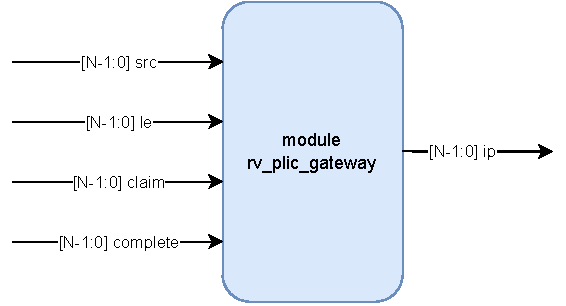
\includegraphics[width=0.95\textwidth]{./fatima_figures/un.drawio.pdf}
  \caption{PLIC Gateway Module.}
  \label{fig:plic_gateway}
\end{figure}

The interrupt gateways in the platform level interrupt controller are responsible for converting global interrupt signals into a common interrupt request format, and for controlling the flow of interrupt requests to the PLIC core. At most one interrupt request per interrupt source can be pending in the PLIC core at any time and it can be indicated by setting the source’s interrupt pending bit. After receiving notification that the interrupt handler servicing the previous interrupt request from the same source has completed, the gateway forwards a new interrupt request to the PLIC core. If the global interrupt source uses level-sensitive interrupts, the gateway will convert the first assertion of the interrupt level into an interrupt request, but thereafter the gateway will not forward an additional interrupt request until it receives an interrupt completion message. If the interrupt is level-triggered and the interrupt is still asserted, a new interrupt request will be forwarded to the PLIC core on receiving an interrupt completion message. The gateway does not have the facility to retract an interrupt request once forwarded to the PLIC core. If a level-sensitive interrupt source de-asserts the interrupt after the PLIC core accepts the request and before the interrupt is serviced, the interrupt request remains present in the IP bit of the PLIC core and will be serviced by a handler, which will then have to determine that the interrupt device no longer requires service. If the global interrupt source was edge-triggered, the gateway will convert the first matching signal edge into an interrupt request. Depending on the design of the device and the interrupt handler, in between sending an interrupt request and receiving notice of its handler’s completion, the gateway might either ignore additional matching edges or increment a counter of pending interrupts. In either case, the next interrupt request will not be forwarded to the PLIC core until the previous completion message has been received. If the gateway has a pending interrupt counter, the counter will be decremented when the interrupt request is accepted by the PLIC.\\

\subsection{PLIC TARGET}
The figure \ref{fig:plic_target} shows the block diagram of module of the PLIC Target.\\

\begin{figure}[h]
  \centering
  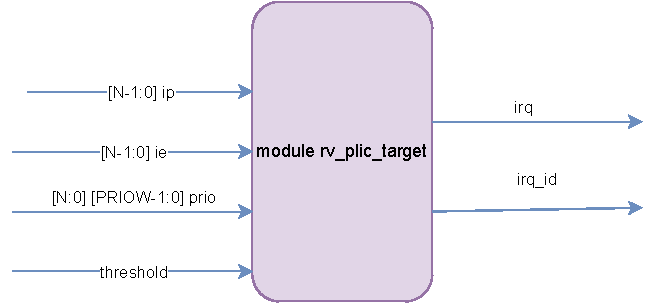
\includegraphics[width=0.95\textwidth]{./fatima_figures/target.drawio.pdf}
  \caption{PLIC Target Module.}
  \label{fig:plic_target}
\end{figure}

The PLIC target deal with the interrupt pending bit, interrupt enable bit, interrupt priority and threshold.\\

The current status of the interrupts pending in the PLIC core can be read from the interrupt pending register. \\

Each target has a vector of interrupt enable (IE) bits, one per interrupt source. The target will not receive interrupts from sources that are disabled. Each global interrupt can be enabled by setting the corresponding bit in the enables register. The IE bits for a single target should be packed together as a bit vector in platform-specific memory-mapped control registers to support rapid context switching of the IE bits for a target. IE bits are WARL fields that can be hardwired to either 0 or 1. Bit 0 of enable register 0 represents the non-existent interrupt ID 0 and is hardwired to 0. \\

The PLIC supports interrupt priorities, that is each PLIC interrupt source can be assigned a priority by writing to its memory-mapped source priority register. A priority value of 0 is reserved to mean never interrupt and effectively disables the interrupt. Priority 1 is the lowest active priority while the maximum level of priority is defined by the max priority parameter. Ties between global interrupts of the same priority are broken by the Interrupt ID; interrupts with the lowest ID have the highest effective priority.\\

The threshold priority level is set via the Priority Threshold Register. An interrupt line with a priority less than the threshold, is masked. As an example, a threshold value of zero permits all interrupts with non-zero priority.\\

\subsection{PLIC Register Map}
The figure \ref{fig:plic_RegMap} shows the block diagram of module of the PLIC Target.\\

\begin{figure}[h!]
  \centering
  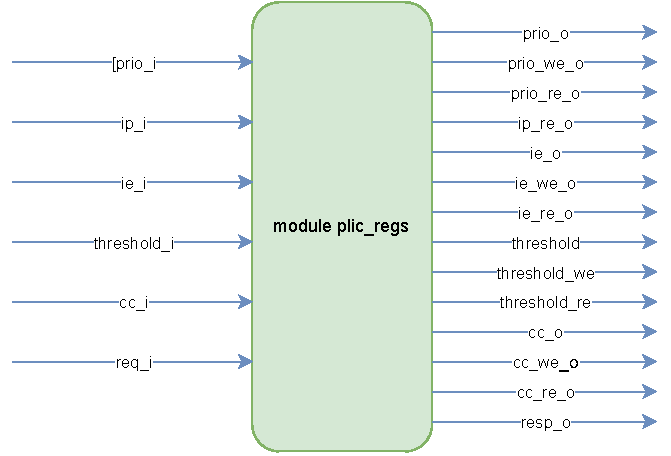
\includegraphics[width=0.95\textwidth]{./fatima_figures/regmap.drawio.pdf}
  \caption{PLIC Target Module.}
  \label{fig:plic_RegMap}
\end{figure}

The register map for the PLIC control registers is shown in table \ref{table:regmap}

\begin{table}[h!]
\centering
 \begin{tabular}{||p{3cm} p{1.5cm} p{1.5cm} p{1.5cm} p{5cm}||} 
 \hline
 \rowcolor{gray}
 Register-Name & Offset(hex) & Size(Bits) & Reset(hex) & Description  \\ [0.5ex] 
 \hline\hline
 \rowcolor{lightgray}
 source priority-0 & 0X0 & 24 & 0X0 & Register holds the priority value of the respective interrupt source\\ 
 \rowcolor{gray}
 source priority-1 & 0X4 & 24 & 0X0 & \\ 
 \rowcolor{lightgray}
 ... & ... & ... & ... & \\
 \rowcolor{gray}
 source priority-31 & 0X7C & 24 & 0X0 & \\ 
 \rowcolor{lightgray}
 source pending & 0X1000 & 32 & 0X0 & Register holds the pending interrupt bits for upto 32 sources in a single register\\
 \rowcolor{gray}
 target enables & 0X2000 & 32 & 0X0 & Register holds the interrupt enable bits for upto 32 sources in a single register\\
 \rowcolor{lightgray}
 target threshold & 0X200000 & 32 & 0X0 & Register holds the priority threshold of the respective target\\
 \rowcolor{gray}
 target claim & 0X200004 & 32 & 0X0 & Register holds interrupt claim/completion information for the respective target\\ [1ex] 
 \hline
 \end{tabular}
 \caption{PLIC Register Map for all configuration registers}
 \label{table:regmap}
\end{table}

Distribute the project goals into smaller objectives/modules and outline deliverables for each objective. Explain the modules of the project through a system-level block diagram. Students may also mention tools, technologies, and suitability of the method(s) to be employed with justification. In case of a research problem, outline the approaches that will be investigated in the project. ($2-3$ pages)

 % Project Development Methodology/Architecture

% Chapter 6

\chapter{Project Milestones and Deliverables}
\label{Chapter6}

Clear milestones should be defined at the start of the project in the form of a Gantt chart. It is recommended to use excel or some equivalent software to make a Gantt chart. ($1-2$ pages) % Project Milestones and Deliverables

% Chapter 7

\chapter{Block Diagram}
\label{Chapter7}

Draw a block diagram of your project and explain it briefly. ($1$ page) % Block Diagram

% Chapter 8

\chapter{Flow Chart}
\label{Chapter8}

Once interrupt source triggers the interrupt, it then goes to gateway and then gateway will request that interrupt to PLIC Core which is shown in the Figure \ref{fig:flow_chart}. 

\par
After the interrupt is requested to PLIC core, it will then \textbf{alert/notify} target(s). Now the important step comes, after the target has received the interrupt, it will send a signal back to PLIC core that this interrupt is claimed (Also the claim ID). Receiving the claim from target, PLIC will send claim response that this interrupt should be serviced or not. Then the interrupt handler services the that particular interrupt. 


\begin{figure}[h]
  \centering
  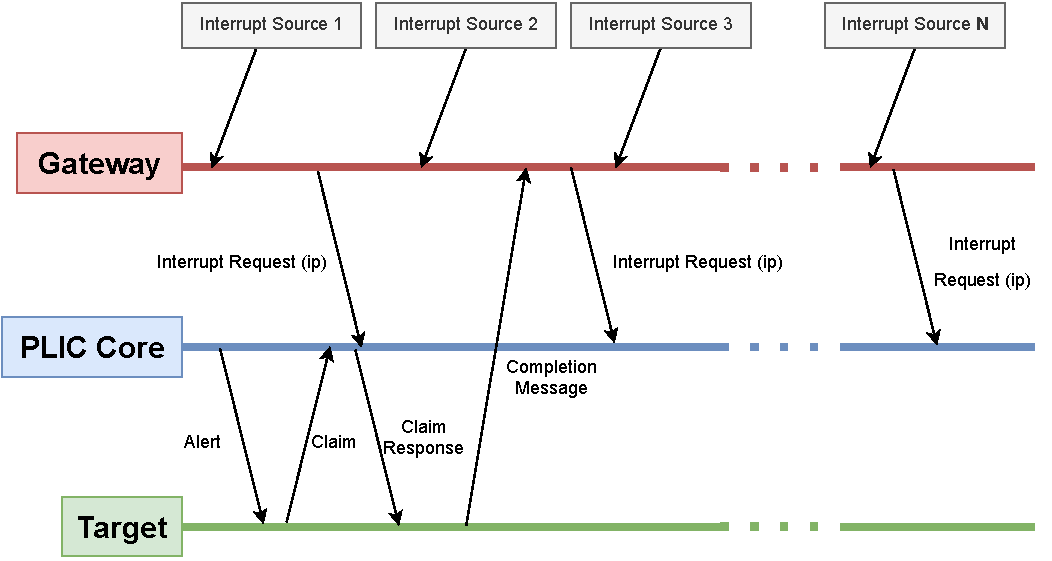
\includegraphics[width=1\textwidth]{F:/FYP/flow_chart.pdf}
  \caption{Flow Chart.}
  \label{fig:flow_chart}
\end{figure}


Finally, the interrupt completion message will be sent to gateway that this interrupt is completed and no need to send any other interrupt from that source. So is the case with all other pending interrupts from other sources.

 % Flow Chart

% Chapter 9

\chapter{Work Division}
\label{Chapter9}

Clear work division among group members must be indicated. ($1$ page) % Work Division

% Chapter 10

\chapter{Costing}
\label{Chapter10}

This project requires quite low budget becaue it is 60 to 70 percent software based. The only hardware required is FPGA.

\begin{center}

\begin{tabular}{|c|c|c|} 
 \hline
Sr No. & Device Name & Software Name \\ [0.5ex] 
 \hline
 1 & Xilinx's Nexys A7 FPGA & xc7a100tcsg324-1 \\ [1ex]
 \hline
\end{tabular}

\end{center}

Rest of the 30 to 40 percent project will be hardware based where Verification of the project will be done on test benches as well as FPGA. % Costing

%% ----------------------------------------------------------------
\appendix
\input{./Chapters/Introduction to Latex}	% For students' reference only. Do not include this file in your final synopsis by commenting out or omitting this bit.

%% ----------------------------------------------------------------
\addtocontents{toc}{\vspace{2em}}  % Add a gap in the Contents, for aesthetics
\backmatter

\bibliographystyle{plainnat}  % Use "unsrtnat" BibTeX style for formatting the references

\bibliography{references}  % The references information is stored in the file named "references.bib"

\end{document}  % The End
%% ----------------------------------------------------------------
